%Schriftart Format
\documentclass{article}
\usepackage[english]{babel}
\usepackage[utf8]{inputenc}
\usepackage[T1]{fontenc}
\usepackage{geometry}
\geometry{a4paper, portrait, margin=30mm, headsep= 32pt , headheight = 19pt, footskip = 40 pt}
\usepackage[]{placeins}
\usepackage{hyperref}

\usepackage[bottom]{footmisc} 


%Grafik:
\usepackage{graphicx}


%Kopfzeile:
\usepackage{fancyhdr}
\pagestyle{fancy}
\fancyhf{}
\fancyhead[L]{\Large ZK-48}
\fancyhead[C]{\Large Documentation}
\fancyhead[R]{\Large Page \thepage}
\cfoot{
\includegraphics[scale=0.06]{./Figures/zk_48_logo.png}}

\setlength{\footskip}{40pt}

%Formeln:
\usepackage{amsmath, amsthm, amssymb}

\usepackage{cleveref}

%Code-darstellen:
\usepackage{listingsutf8}
\usepackage[numbered,framed]{matlab-prettifier}
\lstset{language=Python}
\lstset{literate=
  {á}{{\'a}}1 {é}{{\'e}}1 {í}{{\'i}}1 {ó}{{\'o}}1 {ú}{{\'u}}1
  {Á}{{\'A}}1 {É}{{\'E}}1 {Í}{{\'I}}1 {Ó}{{\'O}}1 {Ú}{{\'U}}1
  {à}{{\`a}}1 {è}{{\`e}}1 {ì}{{\`i}}1 {ò}{{\`o}}1 {ù}{{\`u}}1
  {À}{{\`A}}1 {È}{{\'E}}1 {Ì}{{\`I}}1 {Ò}{{\`O}}1 {Ù}{{\`U}}1
  {ä}{{\"a}}1 {ë}{{\"e}}1 {ï}{{\"i}}1 {ö}{{\"o}}1 {ü}{{\"u}}1
  {Ä}{{\"A}}1 {Ë}{{\"E}}1 {Ï}{{\"I}}1 {Ö}{{\"O}}1 {Ü}{{\"U}}1
  {â}{{\^a}}1 {ê}{{\^e}}1 {î}{{\^i}}1 {ô}{{\^o}}1 {û}{{\^u}}1
  {Â}{{\^A}}1 {Ê}{{\^E}}1 {Î}{{\^I}}1 {Ô}{{\^O}}1 {Û}{{\^U}}1
  {ã}{{\~a}}1 {ẽ}{{\~e}}1 {ĩ}{{\~i}}1 {õ}{{\~o}}1 {ũ}{{\~u}}1
  {Ã}{{\~A}}1 {Ẽ}{{\~E}}1 {Ĩ}{{\~I}}1 {Õ}{{\~O}}1 {Ũ}{{\~U}}1
  {œ}{{\oe}}1 {Œ}{{\OE}}1 {æ}{{\ae}}1 {Æ}{{\AE}}1 {ß}{{\ss}}1
  {ű}{{\H{u}}}1 {Ű}{{\H{U}}}1 {ő}{{\H{o}}}1 {Ő}{{\H{O}}}1
  {ç}{{\c c}}1 {Ç}{{\c C}}1 {ø}{{\o}}1 {å}{{\r a}}1 {Å}{{\r A}}1
  {€}{{\euro}}1 {£}{{\pounds}}1 {«}{{\guillemotleft}}1
  {»}{{\guillemotright}}1 {ñ}{{\~n}}1 {Ñ}{{\~N}}1 {¿}{{?`}}1 {¡}{{!`}}1 
}

\usepackage{float}
\usepackage{siunitx}


\makeatletter
\renewcommand\paragraph{\@startsection{paragraph}{4}{\z@}%
            {-2.5ex\@plus -1ex \@minus -.25ex}%
            {1.25ex \@plus .25ex}%
            {\normalfont\normalsize\bfseries}}
\makeatother
\setcounter{secnumdepth}{4} % how many sectioning levels to assign numbers to
\setcounter{tocdepth}{4}    % how many sectioning levels to show in ToC
\crefname{paragraph}{paragraph}{paragraphs}
\Crefname{paragraph}{Paragraph}{Paragraphs}
\begin{document}

\begin{titlepage}
\begin{center}
\vspace*{1cm}

\includegraphics[width=2cm]{./Figures/zk_48_logo.png}
\vspace*{1cm}

\Huge {Technical Documentation\\} 
\vspace*{1cm}
\Huge{\textbf{48 Output Wired and Programmable\\ Pyrotechnic Ignition System\\ based on the ATTINY 861\\}}
\vspace*{0.5cm} 
\Large{by Markus K. \textit{alias inimodo}}
\vspace*{0.5cm}

\Large{2023}
\end{center}
\end{titlepage}

\pagebreak 

\tableofcontents

\pagebreak

\section{Introduction}
The ZK-48 (German "Zündkasten 48 Ausgänge") ignition system was developed because there are no affordable cheap programmable systems. The goal is a low cost yet reliable and robust device that works in any condition. This document provides all information surrounding this project and anyone with basic knowledge in electronics should be able to rebuild it. Although this should not be viewed as an instruction on how to build this device, but the author hopes it is useful anyway to a pyrotechnic and or electronics enthusiast. The finished device is shown in \Cref{fig:complete_with_trig_and_mod} with the trigger on the right and one module on the left.

\begin{figure}[!ht]
    \centering
    \includegraphics[width=15cm]{./Figures/complete_with_trig_and_mod.JPG}
    \caption{The resulting complete system with igniter and some modules.}
    \label{fig:complete_with_trig_and_mod}     
\end{figure}

\pagebreak

\section{Hardware}
\label{Hardware}

\subsection{Concept}
\label{Concept}
The device is divided into three units: controller, trigger and modules (See \Cref{fig:concept}). The controller is the center piece, that houses the micro controller which is a ATTINY 861\footnote{\url{https://www.mouser.com/datasheet/2/268/Atmel_2588_8_bit_AVR_Microcontrollers_tinyAVR_ATti-1315472.pdf}} from Atmel. On board the controller are the main on/off key-switch, the arm switch,a USB port for programming, status LEDs and connectors for the trigger and modules. The trigger is connected by a $15m$ cable to the controller and has mounted a arm switch and the trigger button. There are six modules and each module is able to ignite eight bridge wire detonators (A-Type Only). The modules are also connected by cable to the controller. Two different cable lengths were used for the modules: 3x $4m$ and 3x $8m$. Therefore the complete system is capable of setting of 48 detonators.

\begin{figure}[!ht]
    \centering
    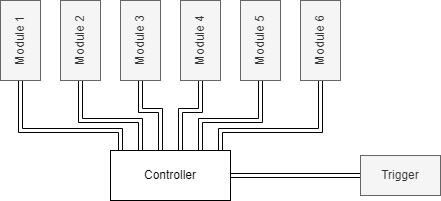
\includegraphics[width=10cm]{./Figures/concept.png}
    \caption{Basic layout of the three components controller, trigger and modules.}
    \label{fig:concept}     
\end{figure}

\noindent The system operates by the fire-and-forget principle, by which the user arms both the controller and the trigger and after pressing the trigger button the controller will automatically ignite the firework in the programmed sequence. No user input is needed after setting off. When the trigger is pressed the system goes into a $10s$ delay phase in order for the user to get to safety. After the delay phase is finished, the ignition phase is entered, where the programmed sequence will play through until the predetermined endpoint is reached. The trigger can be replaced with a RF-trigger although this is not recommend due safety and legal concerns in some countries. The delay period also serves as a fail safe, because if the system is triggered by accident, the user is able to abort the start by disarming the system. During the ignition phase it is also possible to halt the program by disarming the system, although re-triggering will go through the delay phase again.\\

\noindent The ignition sequence is programmed by USB via serial communication(See \cref{USB Connection}). Programming the sequence can be accomplished by directly connecting to the serial port and typing the commands by hand or by using the Software provided(See \cref{Software}).\\

\noindent As the device is most likely placed in open-air field there is no way for it to be power by mains power, therefore it has to be powered by batteries. However, the usage of rechargeable batteries or LiPo-batteries was not desirable for this project, due cost issues and the additional requirement of protection circuits. A better alternative was found by using common $5V$ powerbanks for smart phones. Those already provide steady $5V$ with build-in protective mechanisms. Furthermore, nowadays many people use powerbanks and if the user forgets to charge or forgets the powerbank altogether, there is a high chance some will be able to provide one as replacement. A powerbank can be charged by a simple micro USB cable which is also very common and removes the need for a specialized charger.





\pagebreak

\subsection{Components}
As already explained in \cref{Concept}, the device is split into three parts. This section will explore each part separately by looking into the design choices that were made. Although the controller is described as one unit, in reality consist  of to distinct circuits. One is the ignition voltage generator (See \cref{Ignition Voltage Generator}) which is responsible for generating the voltage/charge that is necessary for setting off the bridge wire detonators. The other circuit is the control logic that does the controlling (See \cref{Controller}).


\subsubsection{Ignition Voltage Generator}
\label{Ignition Voltage Generator}



\noindent The step-up convert shown in \Cref{fig:ivg_circuit} works by the basic principle of a step-up/boost converter by storing energy in form of a magnetic field inside a inductor and releasing the energy as a current into a capacitor. Repeat this process at high frequency and a higher voltage is created at the output compared to the input voltage. For a better explanation see the document about this topic by \textit{Texas-Instruments}\footnote{\url{https://www.ti.com/lit/an/snva731/snva731.pdf}}.


\paragraph{The Circuit}

\begin{figure}[!ht]
    \centering
    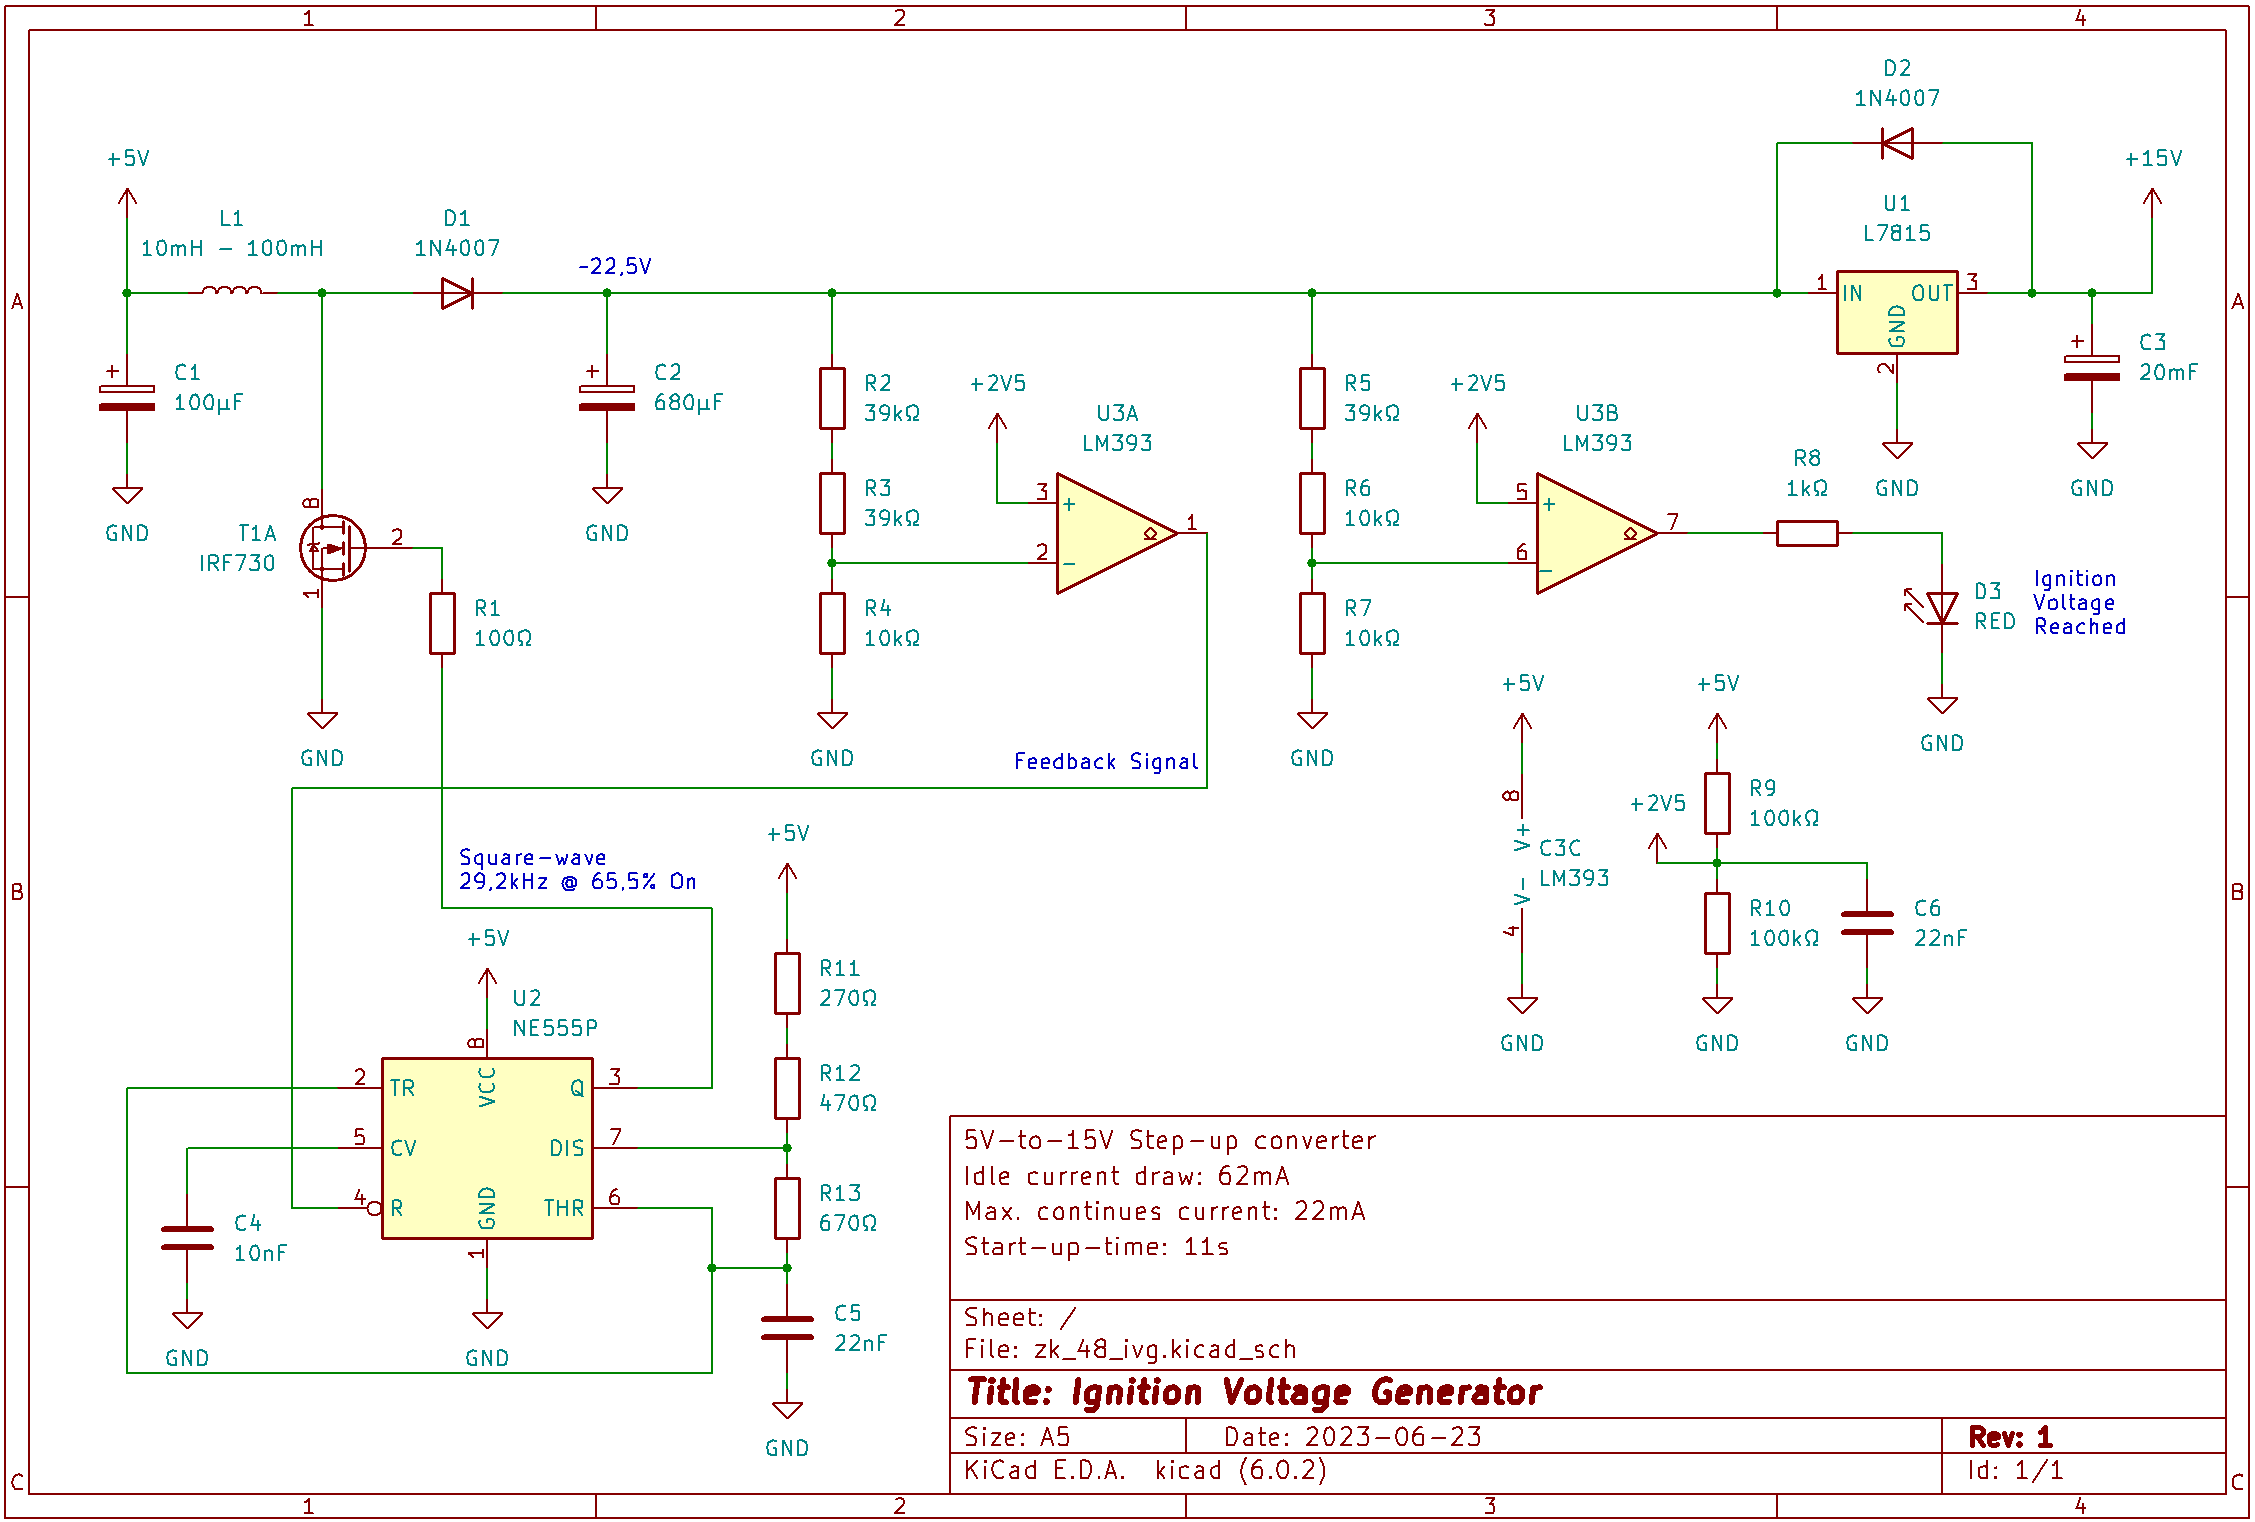
\includegraphics[width=15cm]{./Figures/ivg_circuit.png}
    \caption{Circuit of the step-up converter that generates 15V DC for the ignition voltage}
    \label{fig:ivg_circuit}     
\end{figure}

\pagebreak

\paragraph{How does the circuit work?}

\noindent The circuit shown in \Cref{fig:ivg_circuit} is made up of the popular NE555\footnote{\url{ https://www.ti.com/lit/ds/symlink/ne555.pdf}} used as oscillator, the dual comparator LM393\footnote{\url{https://www.ti.com/lit/ds/symlink/lm393.pdf}} and a fixed linear $15V$ voltage regulator L7815\footnote{\url{https://www.st.com/resource/en/datasheet/l78.pdf}}. The NE555 wired as a square wave oscillator generates a $29,2kHz$ $5V_{pp}$ signal with a $65,5\% $ on-time. This signal is used to drive the IRF730\footnote{\url{https://www.vishay.com/docs/91047/91047.pdf}} N-channel MOSFET which switches the current through the inductor $L1$ and therefore charges the capacitor $C2$. We shall name this voltage the intermediate voltage.\\

\noindent Through a voltage divider the voltage at $C2$ is stepped down by a factor of $\frac{1}{9}$ and compared to a $2,5V$ reference voltage by $U3A$. This results in a $5V$ output signal at $U3A$ if the capacitor $C2$ voltage is lower than $22,5V$. This signal is called the feedback signal with turns off the NE555 if the intermediate voltage has reached $22,5V$. A schmitt-trigger was intentionally not used, because this would result in a oscillating turning off and on of the feedback signal which is undesirable in this configuration. \\

\noindent The intermediate voltage is then converted by the L7815 to stable $15V$ which charges the large $20mF$ ignition capacitor $C3$.  This voltage is called the ignition voltage.\Cref{eq:power_in_system} calculates the energy stored in the complete system with all six modules connected (Thus the total capacitance is $26mF$, but read more in \Cref{Module}) which equates to around $3J$ and therefore does not present any harm or danger to life\footnote{\url{https://www.ehss.vt.edu/programs/ELR_capacitors.php}}. Touching fully charged capacitors with sweaty hands did not result in any shock or pain.\\

\begin{equation}
W_{el}=\frac{U^2 \cdot C_{tot}}{2}=\frac{(15V)^2 \cdot 26mF}{2}=2,925J
\label{eq:power_in_system}
\end{equation}\\

\noindent The second comparator $U3B$ in the LM393 package was used to turn on a red LED $D3$ whose purpose is to indicate whether the intermediate voltage is bigger than $14,75V$. This shows the user if the system is ready for operation and if a ignition voltage is present.\\


\noindent \small{\textit{Note: Please note that the ignition voltage generator was designed by the author and is by no means ideal nor optimized. This was the first attempt at creating a step-up convert from scratch with components that were on hand. It does the job well but any bought step-up convert will do just fine and most likely better.}}\\

\pagebreak

\subsubsection{Controller}
\label{Controller}
\paragraph{Circuit}
\paragraph{Housing}

\subsubsection{Trigger}
\paragraph{Circuit}
\paragraph{Housing}

\subsubsection{Module}
\label{Module}
\paragraph{Circuit}
\paragraph{Housing}


\section{Firmware}
\label{Firmware}

\subsubsection{USB Connection}
\label{USB Connection}
\paragraph{Program Mode}
\paragraph{Commands}


\section{Software}
\label{Software}

\pagebreak

\section{Recognitions}
\label{Recognitions}
All circuits were drawn with the help of $KiCad\ 6.0$\footnote{\url{https://www.kicad.org/}}\\

\noindent All flowcharts and diagrams were drawn with the help of $Drawio$\footnote{\url{https://app.diagrams.net/}}



\end{document}
